\chapter{Design of a LoRa-Based Vehicular Mesh Network for Cooperative Driver Assistance}

\section{Top-level Overview}

The proposed LoRa-based V2V mesh system uses a \textbf{three-layer architecture} so that application
features, network behavior, and radio transmission are kept separate. Keeping the system layered like
this makes it easier to build, test, and modify, while still supporting distributed safety-message
dissemination between vehicles over a constrained long-range wireless link.

The \textbf{Application Layer} is where vehicle services create and use messages. It generates outbound
traffic for neighboring vehicles and processes inbound messages delivered by the lower layers. We keep
this layer independent of routing policies and radio details, so service-level logic stays clean.

The \textbf{Network Layer} is the control core of the system. It manages delivery and forwarding
decisions by adding network metadata (such as hop counts, timestamps, and originator identifiers),
deciding whether a received packet should be delivered locally and/or forwarded, suppressing duplicates
to save channel usage, and scheduling relay timing to reduce contention and collisions. Keeping these
policies in one place also makes it easier to test and tune forwarding behavior.

The \textbf{Link Layer} sits at the radio boundary and handles actual transmission and reception on the
LoRa hardware. It packetizes serialized messages, manages radio state changes and channel sensing, and can
optionally use selective acknowledgment and retry for reliability. Since hardware details are contained here,
the upper layers do not need to change if the physical backend changes.

In normal operation, application payloads go down the stack to be transmitted, and received radio frames go
up through the Link and Network layers before reaching the Application Layer. To support both real hardware
runs and simulation-based testing, the Network Layer is kept hardware-independent using a clear abstract
interface to the Link Layer. This lets the same logic run either with real radio devices or with a
software-based channel simulator for controlled validation. The overall layering and data flow are shown in
Fig.~\ref{fig:system_architecture}.

\begin{figure}[h]
    \centering
    
\includegraphics[width=0.45\textwidth]{"assets/architecture/top_level.jpg"}
    \caption{Three-layer architecture of the LoRa-based V2V mesh system, showing the Application, Network,
    and Link layers, the message flow for transmission and reception, peer vehicles, and the wireless channel.}
    \label{fig:system_architecture}
\end{figure}


\section{Network Layer Architecture}

The network layer acts as the control plane of the proposed LoRa-based V2V mesh system. We designed it as a
portable, hardware-independent core that sits between the application services and the radio-facing
transmission services. Its job is to take locally generated safety data and turn it into network frames that
can be disseminated, to check received frames against the propagation policy, and to control rebroadcasting so
that reliability improves without wasting channel time. We do this by keeping clear boundaries that separate
forwarding logic from platform-specific communication and sensing details, so the same network behavior can be
used on embedded devices and in a host-side simulation.

At the transmission boundary, each outgoing frame is a fixed network header followed by application payload
bytes. The header carries message identity, temporal validity, origin context, per-hop transmitter context, and
propagation constraints, so downstream nodes can decide what to do based on self-contained metadata. Using a
fixed header length keeps parsing deterministic and the overhead bounded. The payload limit is set based on the
LoRa frame-size ceiling, so any generated frame is admissible for the physical channel. A unique message
identifier is created by combining the source identity with a local sequence progression. This supports replay
suppression and idempotent handling across multi-hop dissemination.

A key design principle is separating immutable origin metadata from mutable per-hop transmitter metadata.
Origin metadata does not change for the lifetime of a message and represents the initial source state at the
time of creation. Transmitter metadata is updated at every relay and represents the most recent forwarding
node. This separation lets the forwarding logic reason about the overall propagation intent and the local
progress at the same time, which is needed for hold-back scheduling and redundancy suppression in dynamic
vehicular topologies.

Operationally, the data plane has two coordinated paths: synchronous origination and asynchronous
reception-driven forwarding. During origination, the layer checks that the payload is admissible, builds the
network header using local time and mobility context, records the message identity in a duplicate-tracking
structure, and sends a single broadcast frame. During reception, incoming frames are first buffered in a
bounded event queue and then processed by worker execution contexts that handle parsing, policy evaluation,
local delivery, and (if needed) relay scheduling. This separation stops the receive callbacks from becoming
policy bottlenecks and makes the timing more predictable under bursty traffic. The receive-path processing
sequence is shown in Fig.~\ref{fig:network-layer-sequence}.

\begin{figure*}[!t]
\centering
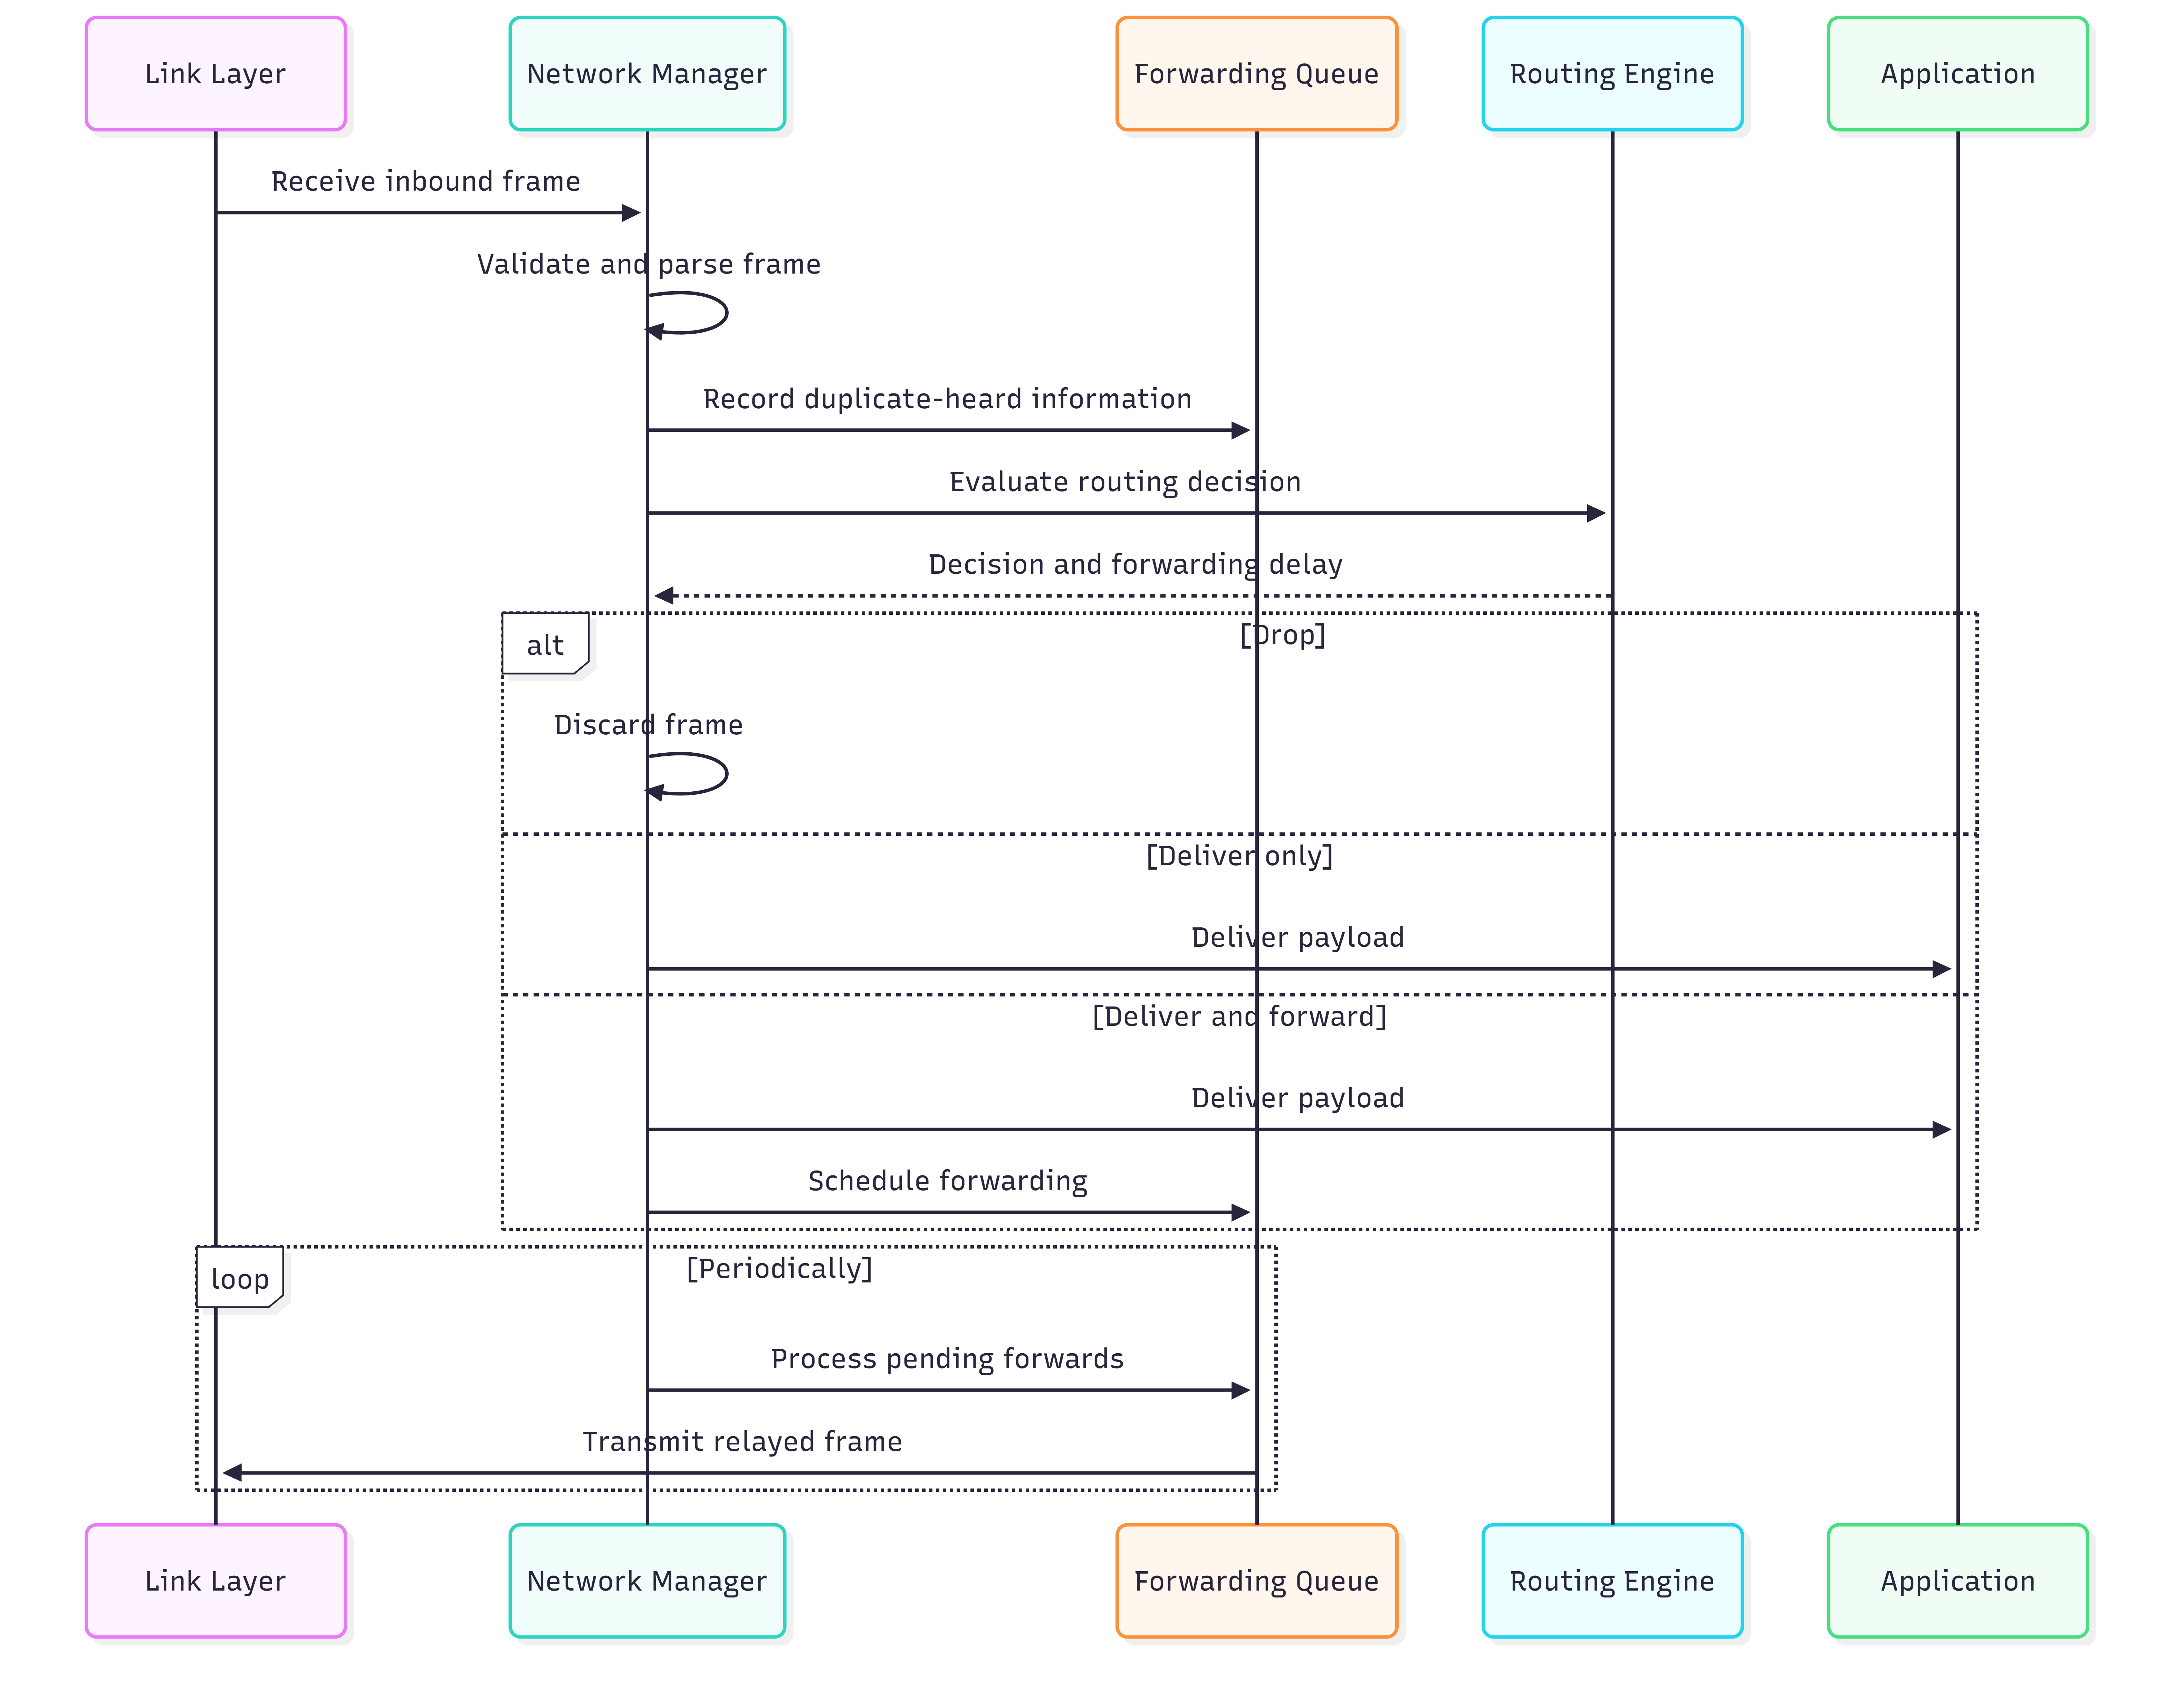
\includegraphics[width=0.95\textwidth]{assets/architecture/Network_layer_seq.png}
\caption{Receive-path sequence of network-layer processing, from link-layer callback ingestion and queueing to
routing evaluation, local delivery, and deferred forwarding.}
\label{fig:network-layer-sequence}
\end{figure*}

Forwarding decisions are made using an ordered evaluation pipeline that prioritizes safety and bounded
propagation. Frames are first screened for temporal expiry, replay status, and remaining hop budget. After
that, we check distance-constrained dissemination and directional eligibility when directional propagation is
requested. Messages that pass these gates become relay candidates, and we assign them a deferred forwarding
delay instead of retransmitting immediately. The delay is computed from a composite estimate of path progress
and link quality, and then adjusted by traffic priority so urgent safety traffic propagates with lower latency
while less critical traffic is naturally delayed. This mechanism implements contention-aware spatial diversity
by encouraging favorable relays to transmit earlier and discouraging simultaneous redundant rebroadcasts. The
ordered decision logic and outcomes are summarized in Fig.~\ref{fig:network-layer-decision}.

\begin{figure*}[!t]
\centering
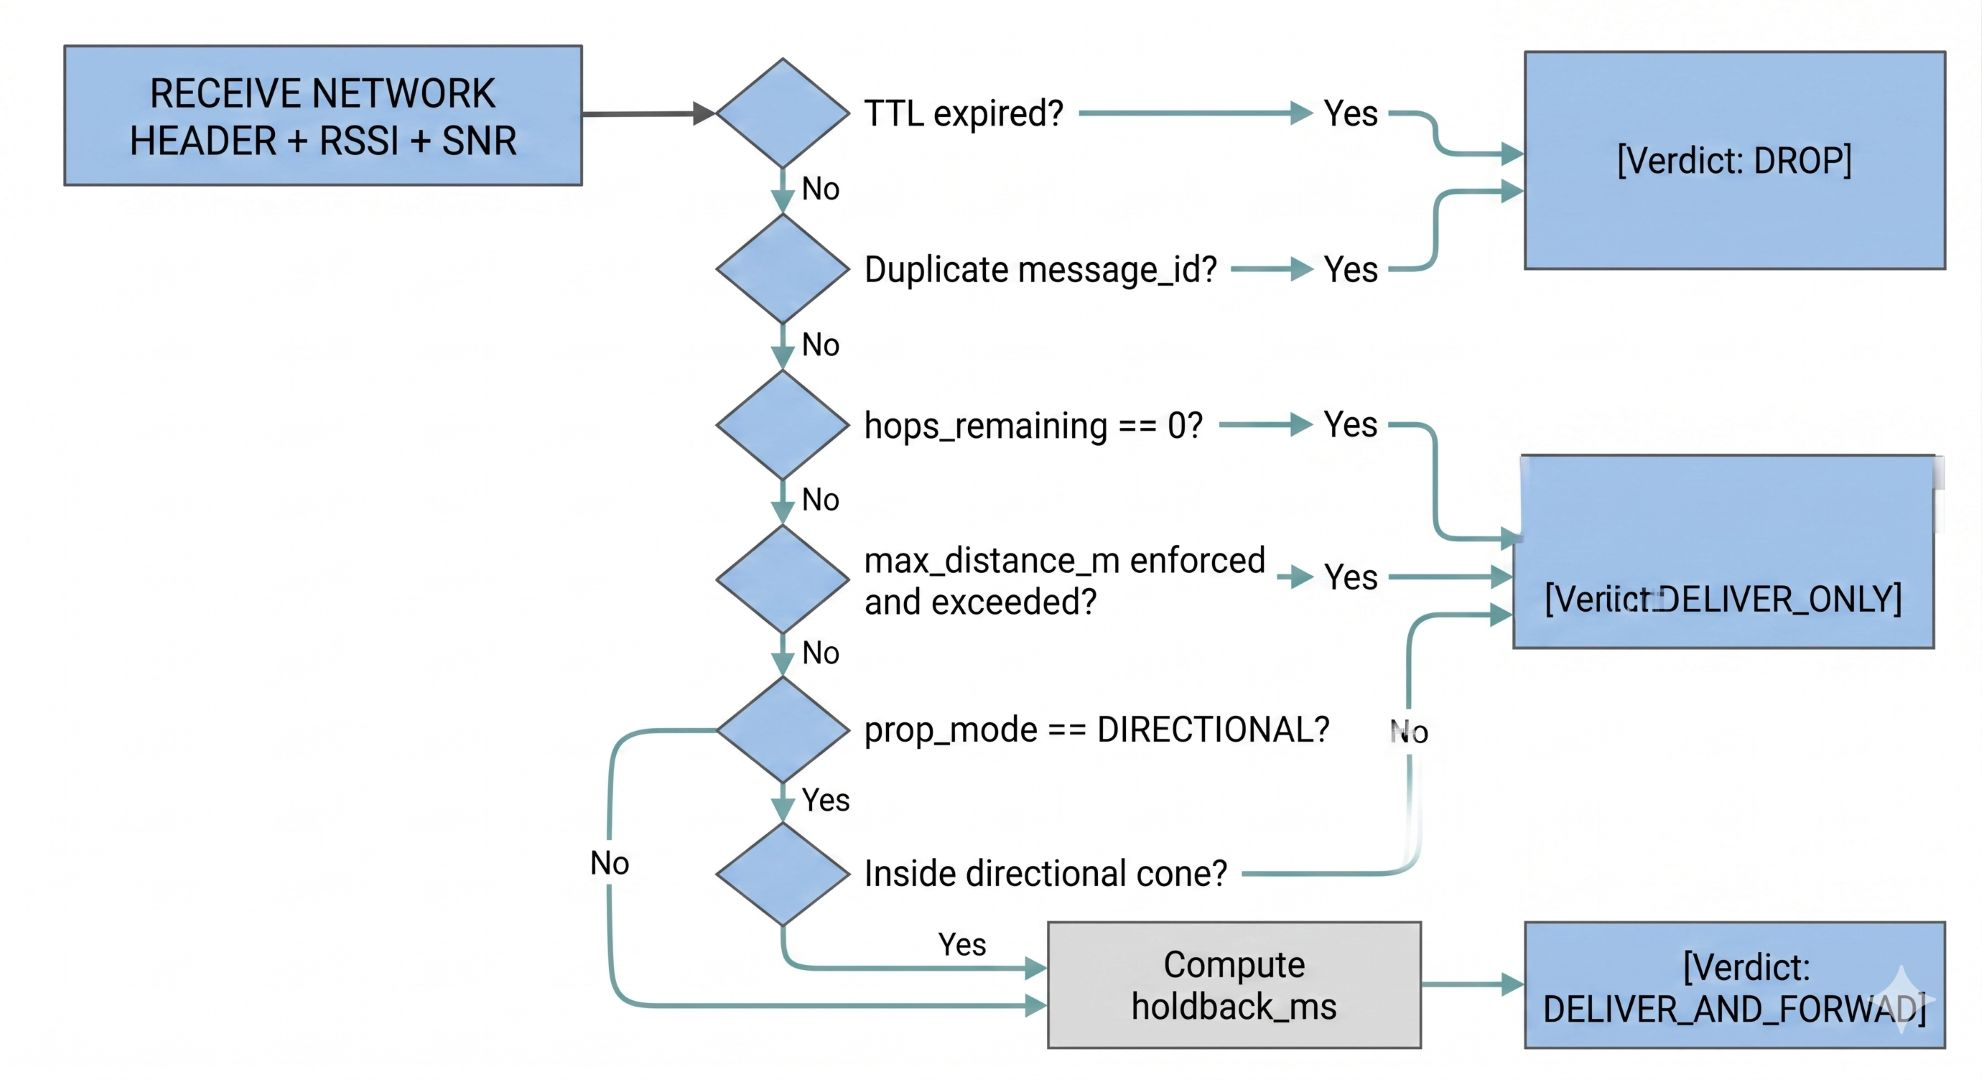
\includegraphics[width=0.6\textwidth]{assets/architecture/network_layer_decision.jpg}
\caption{Network-layer decision pipeline for received frames, showing the ordered checks that determine drop,
deliver-only, or delayed forwarding outcomes.}
\label{fig:network-layer-decision}
\end{figure*}

To further limit broadcast redundancy, the architecture uses two suppression mechanisms. First, duplicate
filtering stops repeated processing and forwarding of message identities that have already been seen. Second,
queued relays can be canceled if later overheard transmissions suggest that upstream progression already
covered what this node would have contributed. This geometric suppression reduces unnecessary retransmissions
without explicit coordination exchanges, which fits bandwidth-constrained and intermittently connected
vehicular channels.

Concurrency management is important for correctness. The network layer uses separate execution contexts for
receive-path processing and timer-driven relay emission, with mutex- and condition-variable-based
synchronization around bounded shared queues and callback handoff state. Lifecycle control is made robust for
repeated start-stop operation, with deterministic initialization, safe termination of background activity, and
clean release of receive handlers during shutdown. Overall, this threading model keeps a clear separation
between ingress handling, routing computation, and deferred transmission timing.

The architecture also exposes bounded configuration controls for duplicate-cache capacity, relay-queue
capacity, receive-queue depth, and forwarding delay limits. These parameters define the operational envelope
for memory consumption, latency, and admission behavior, and they allow systematic trade-off analysis between
responsiveness and channel load. Along with fixed frame-level constraints, this configuration model helps keep
runtime behavior predictable across different hardware targets.

Finally, we embed the same network-layer core in a deterministic simulation runtime to support repeatable
validation under controlled mobility and channel conditions. Each simulated node runs the same logical network
functionality as a deployed node, while a shared virtual clock and event-driven channel model control
transmission timing, reception outcomes, and channel impairments. Since routing and forwarding semantics are
preserved across deployment and simulation, the behavior observed in the lab can be transferred more directly
to field-oriented configurations.



\section{Link Layer Architecture}

The link layer implements the single-hop communication behavior needed by the upper stack, while keeping a
strict boundary from routing and application logic. Its main job is to provide dependable one-hop delivery on a
constrained long-range channel. This includes frame construction, channel access coordination, reception
handling, and energy-aware behavior. In our design, upper layers submit payloads and receive delivery events
through an asynchronous service interface, while all radio-facing behavior stays inside the link layer. This
separation lets forwarding policy and application logic evolve without being tightly coupled to modem-specific
constraints.

The wire format uses a compact fixed-size header followed by a bounded payload region. This keeps parsing
deterministic and makes interoperability across nodes explicit. The header encodes source and destination
identifiers, message classification, sequence numbering, control flags, and payload length. For addressing, we
use node-local unicast identifiers and a dedicated broadcast destination value for one-to-many dissemination.
Sequence and flag metadata support reliability signaling when needed, without adding mandatory overhead for
every traffic class. We also reserve a message type for acknowledgment control traffic, so ACK signaling is not
confused with application-defined data categories.

Medium access control uses a listen-before-send strategy based on channel activity detection. Before sending,
the transmitter checks for channel occupancy and defers when LoRa activity is detected, which reduces
collision probability on a shared medium. If the channel is repeatedly busy, we apply bounded retry behavior
with randomized backoff to reduce synchronization between concurrent transmitters. If the medium stays
unavailable beyond the configured sensing budget, the pending transmission is discarded so latency does not
grow without bound and the queues do not become unstable. Overall, we prefer predictable timing and spectrum
discipline over aggressive persistence. The runtime state transitions are shown in
Fig.~\ref{fig:link-layer-state-machine}.

\begin{figure*}[!t]
\centering
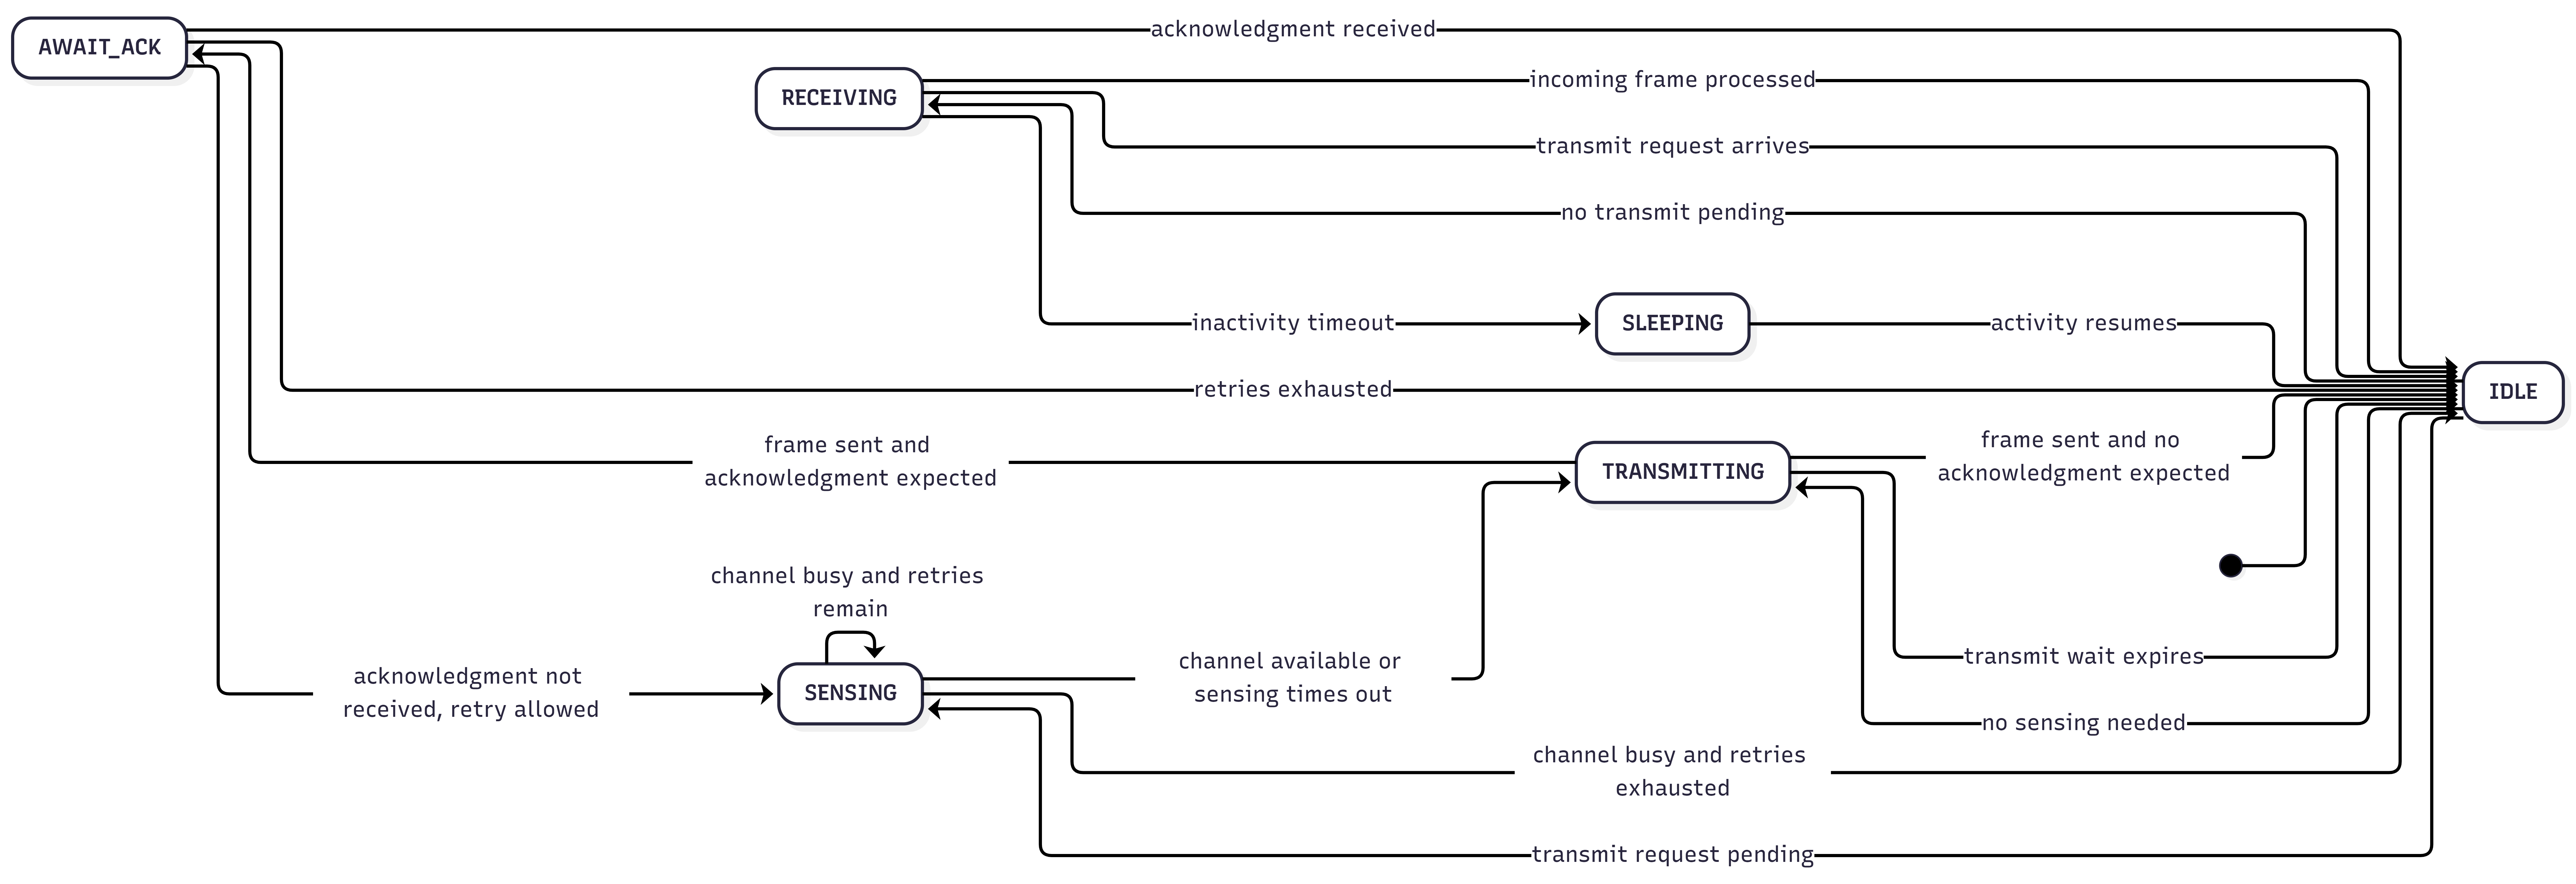
\includegraphics[width=0.95\textwidth]{assets/architecture/link_layer_state_machine.png}
\caption{Link-layer runtime state machine showing transitions among reception, channel activity detection,
transmission wait, acknowledgment wait, sleep control, and idle handling.}
\label{fig:link-layer-state-machine}
\end{figure*}

The transmission workflow combines queued frame dispatch with optional per-frame reliability. Once a frame is
admitted for transmission, it goes through channel sensing and, if the channel is clear, it is transmitted over
the radio interface. For traffic that does not request reliability, we finish once the transmit confirmation is
received. For reliability-enabled traffic, the sender enters a bounded acknowledgment wait phase and checks
incoming acknowledgments against the sequence and addressing context. A valid match ends the transaction and a
positive outcome is reported to the upper layer. If there is a timeout, we do controlled retransmissions up to
the configured maximum, after which the frame is reported as undelivered. This selective reliability model lets
critical safety messages request stronger delivery assurance while keeping lower overhead for noncritical
traffic, as shown in Fig.~\ref{fig:link-layer-sequence}.

\begin{figure*}[!t]
\centering
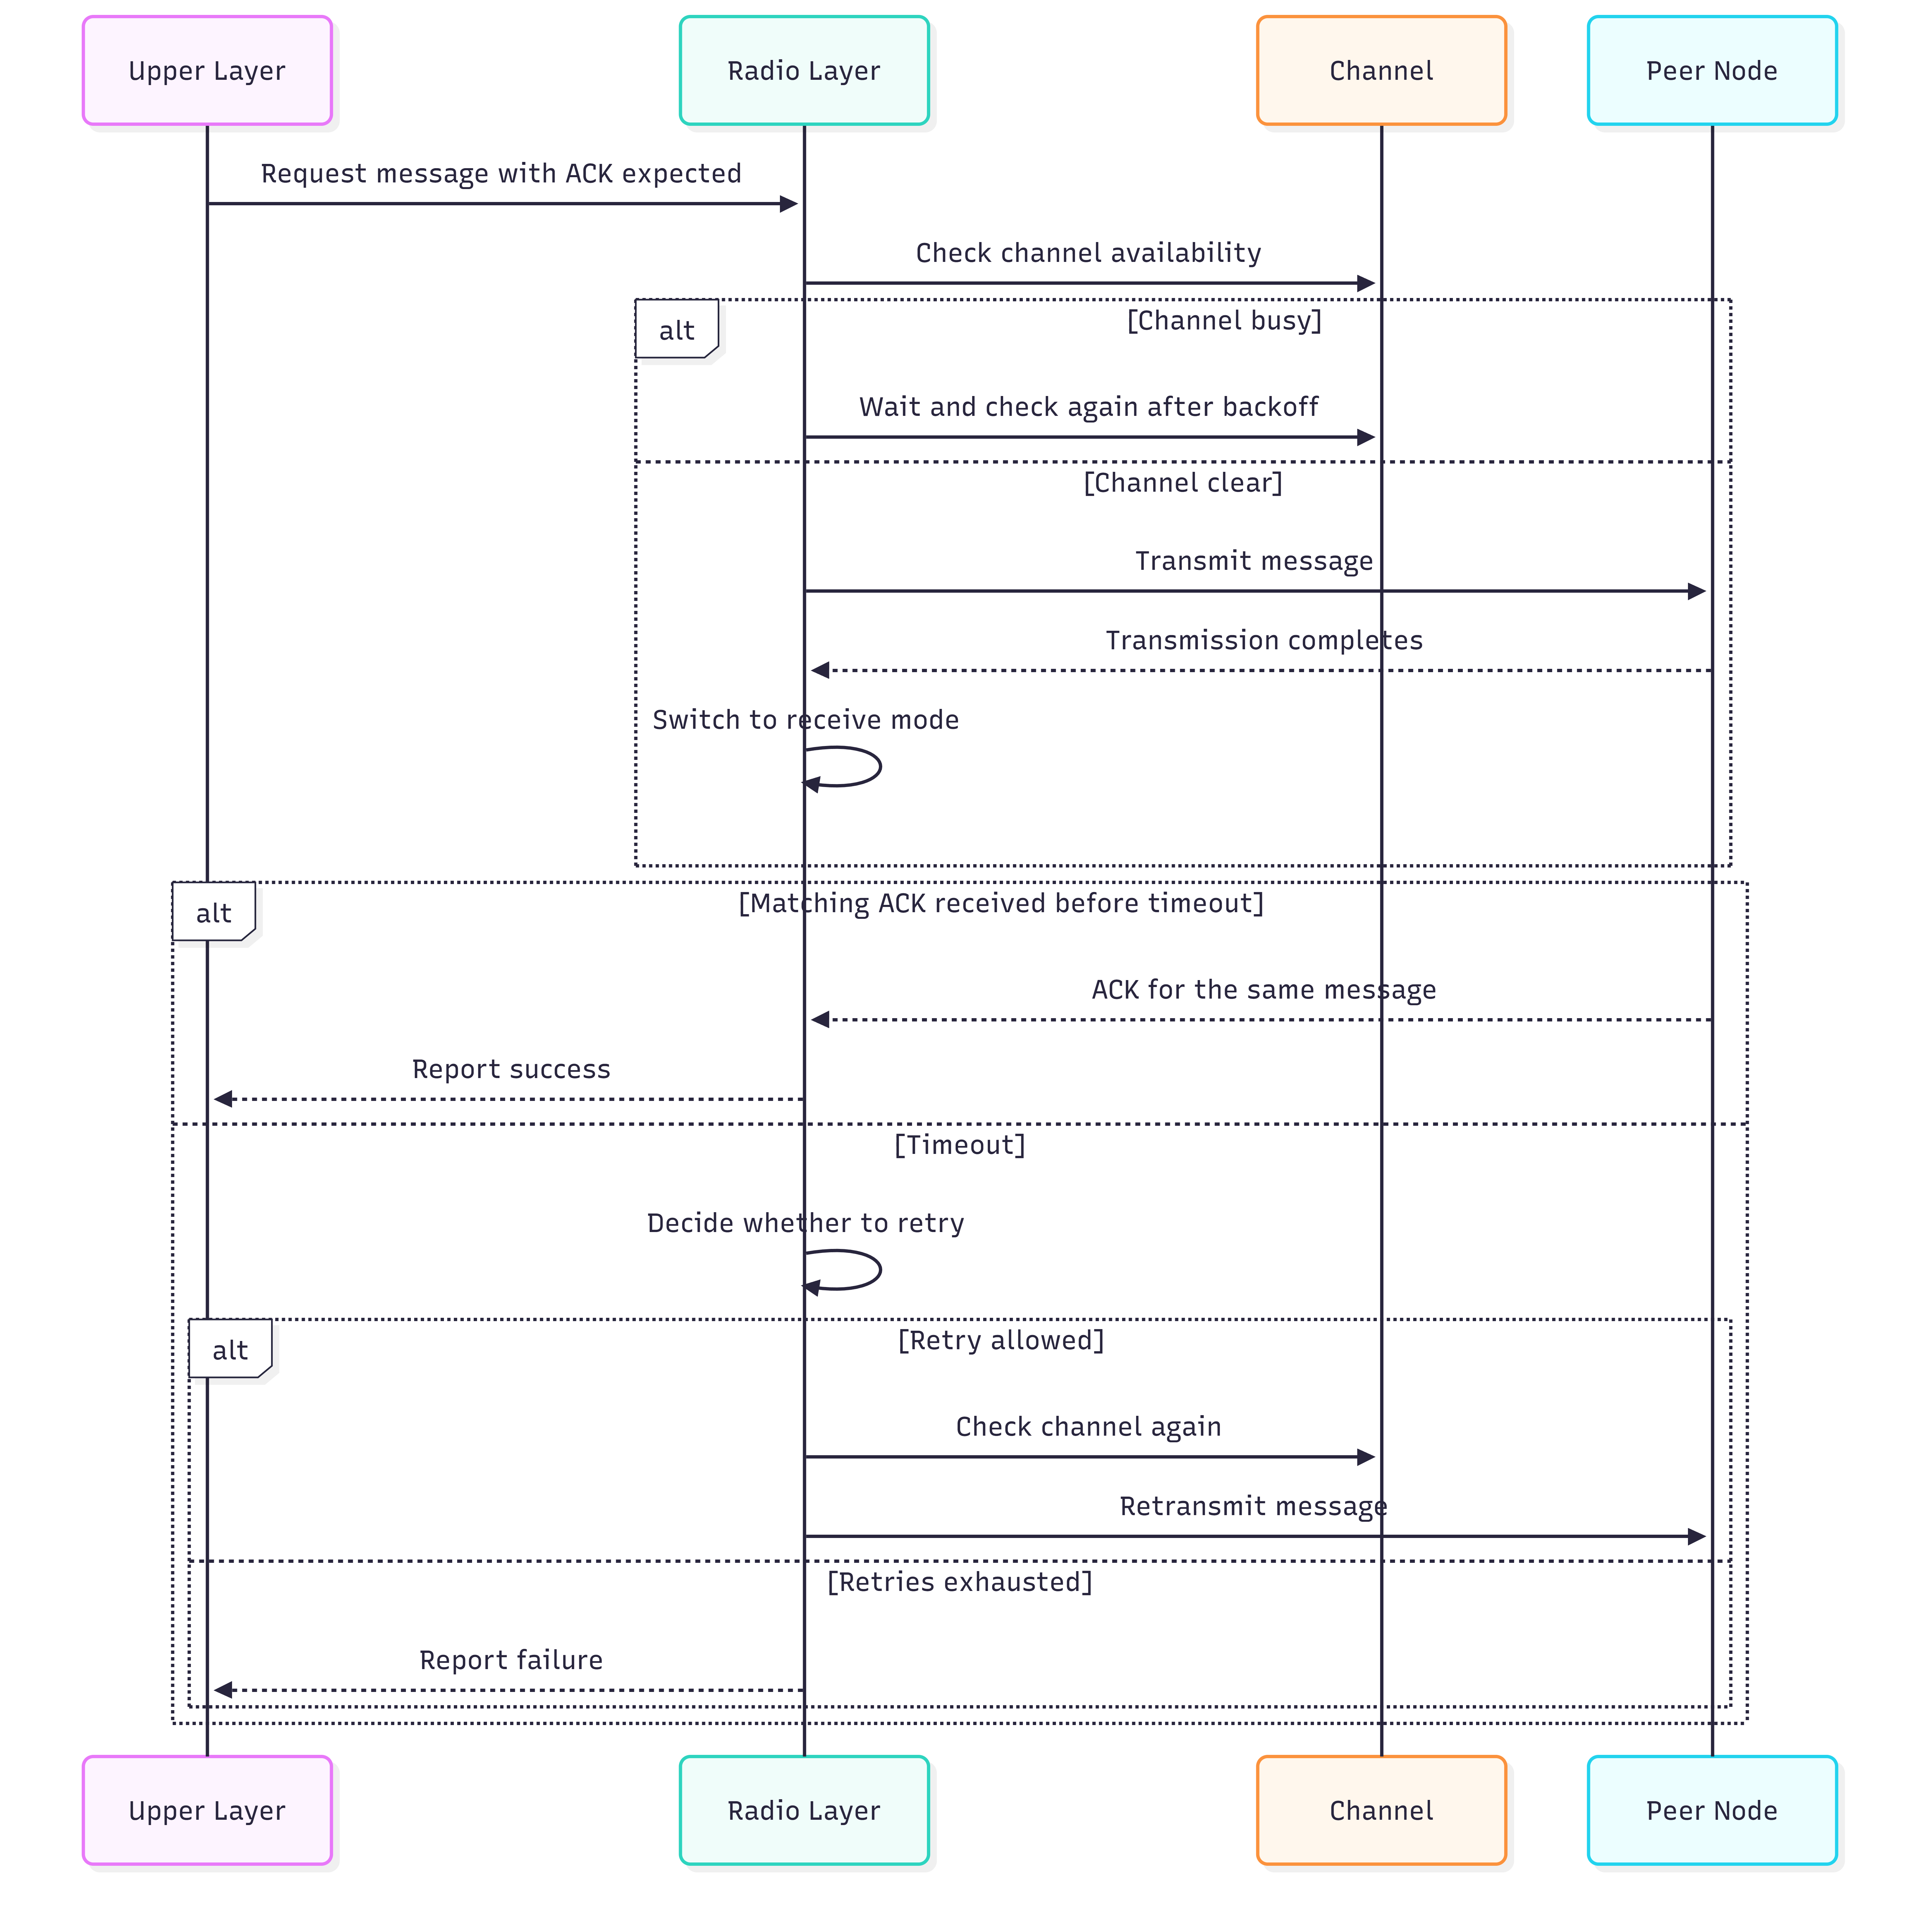
\includegraphics[width=0.7\textwidth]{assets/architecture/link_layer_seq.png}
\caption{Acknowledgment-enabled transmit sequence at the link layer, including CAD-based channel access,
transmission completion handling, ACK validation, timeout detection, and bounded retransmission.}
\label{fig:link-layer-sequence}
\end{figure*}

Inbound processing follows a strict filtering pipeline so upper layers do not have to deal with malformed or
irrelevant traffic. Frames below the minimum valid length are rejected immediately. Valid frames are parsed
and link-quality observations are recorded for neighbor awareness. Destination filtering then removes packets
that are not addressed to the local node or the broadcast group. Pure acknowledgment frames are handled
internally by the reliability subsystem and are not exposed as application payload events. If a received data
frame requested acknowledgment, we generate the corresponding acknowledgment response at link level. Only
after these checks pass do we deliver payload data upward, so upper layers only see semantically meaningful
and policy-compliant traffic.

Energy management is handled through adaptive receive-idle control. The receiver stays active to remain
responsive, but it transitions to a low-power modem state after sustained inactivity. Wake-up is event-driven:
outbound traffic demand or relevant radio interrupt activity restores active operation and normal processing.
This balances readiness and battery efficiency for vehicular platforms that may need to operate for long
intervals without missing important events.

Hardware abstraction is done through a backend interface that separates protocol/state logic from the
transceiver drivers. The link layer uses this interface for channel sensing, transmission, reception,
signal-quality observation, interrupt signaling, and power-state transitions. Because of this, the same
link-layer behavior can run against real radio hardware or controlled test backends without changing the
architecture. This improves portability, supports deterministic validation in the lab, and reduces coupling
between communication policy and platform-specific implementation details.



\section{Techniques}
Forwarding decisions are produced by an ordered evaluation pipeline that prioritizes safety and bounded
propagation. Frames are first screened for temporal expiry, replay status, and residual hop budget, followed
by checks on distance-constrained dissemination and directional eligibility when directional propagation is
requested.

Medium access control follows a listen-before-send strategy based on channel activity detection. Prior to
transmission, the transmitter assesses channel occupancy and defers when LoRa activity is detected, reducing
collision probability under shared medium contention.

This selective reliability model allows critical safety messages to request stronger delivery assurance while
preserving lower overhead for noncritical traffic.

